\documentclass[sigconf]{acmart}

\usepackage{graphicx}
\usepackage{hyperref}
\usepackage{todonotes}

\usepackage{endfloat}
\renewcommand{\efloatseparator}{\mbox{}} % no new page between figures

\usepackage{booktabs} % For formal tables

\settopmatter{printacmref=false} % Removes citation information below abstract
\renewcommand\footnotetextcopyrightpermission[1]{} % removes footnote with conference information in first column
\pagestyle{plain} % removes running headers

\newcommand{\TODO}[1]{\todo[inline]{#1}}
\graphicspath{ {images/} }

\begin{document}



\title{Big Data Analytics in Sports - Soccer}


\author{Rahul Velayutham}
\affiliation{%
  \institution{Indiana University Bloomington}
  \streetaddress{2661 E 7th Street Apt H}
  \city{Bloomington} 
  \state{Indiana} 
  \postcode{47408}
}
\email{rahul.vela@gmail.com.com}

% The default list of authors is too long for headers}
\renewcommand{\shortauthors}{}


\begin{abstract}
Big Data is rapidly becoming a crucial component in the majority of the fields, be it from medicine to software. Big data technologies help in processing humongous amounts of data in a rapid manner while enabling us to achieve results fast and accurately. The impact of Big data in the field of sports, in particular, soccer and how they have helped football clubs evolve their business models and operations from a more hands-on approach to applying complex software and ML models to improve tactics, scouting, and training practices. This study takes a look at the technologies that have been used like MiCoach, Tracab and a look at the leading players like Opta and how the data generated from these companies could be put to use. It is hoped that this study will help demonstrate the importance of Big data in sports, its applications, and avenues for improvement in the field.
\end{abstract}

\keywords{Big Data, Soccer , Scouting}

\maketitle

\section{Introduction}


\section{Big Data in Soccer}

Big Data has become a crucial part of soccer. Data obtained from big data technologies is used to chart training sessions, shape tactics, predict odds for betting and suggest line ups for fantasy premier leagues. Journalists are increasingly using facts obtained from big data to corroborate their stories and often create new stories when normally none could have existed, for example stats may show a player’s ineffective performance could be masked by the good form of the team mates around him. We will now go into a little detail of how all this is done.


\subsection{Big Data in Scouting}

\subsubsection{Introduction}

Two of the biggest commodities in soccer are the clubs and its players. As mentioned previously transfers are now some of the biggest sources of revenue for clubs. Players fetch for as high as 200 million pounds these days\cite{wikipedia}. Also, the quest to find the next big star / the hidden gem against proven expensive players is now a mark of success. Clubs cannot freely go and sign whoever they feel are data monsters, restrictions on the number of players they can sign while at the same time the potential costs that may be involved in the transfer force clubs to make sure the investment they make are the right one. It is recommended to have a look at this article to understand what happens behind the scenes at football clubs when it comes to scouting\cite{2012}.

\subsubsection{Data collection}

Most clubs either have acquired specific companies for scouting for example Arsenal FC acquired paid over 2 million pounds for the US company StatDNA, whose data has since been used to advise their signings. \cite{Outsideoftheboot2000}, and or have scouts who obtain the data themselves. As to how clubs obtain the data, most do not divulge such details to protect their strategies but consensus is that popular sites like opta which analyze matches at real time and release statistics for others to make use of\cite{Optasports2000}. Alternatively, clubs send performance analysts to feeder clubs and they track matches of prospective candidates and create data for themselves.\newline
It is also worth noting that big data has led to only to software development but as well as hardware, for example the Adidas MiCoach a device that tracks metrics and displays it to coaches is used during training and potential scouting sessions. The article mentioned provides an example of how the device was used to realize a gem among a batch of superstars\cite{2000}.

\subsubsection{Data Processing}

Most articles only explain in theory how they go on about processing the data and even fewer talk about the technical aspect behind it. Corroborating from different sources \cite{Rein2016}\cite{Luca20000}\cite{Outsideoftheboot2000} a general theoretical summary can be given, In the case of obtaining data from say the internet i.e., mine data from free sites like squawka, whoscored, opta. Data warehousing technologies like pig, Hadoop etc, can be used. Parsing the XML, one can store this data and applying meaningful ML algorithms with defined parameters to filter players. For example, we can mine the data for fields like chances created, distance covered etc for a league and then filter out say midfielders and chances created in order to find the next best attacking midfielder.\newline
For clubs generating their own data, real time analysis of videos using advanced image processing technologies in tandem with their own hands on analysis they could generate data and store it again or say CSV files. These files then could be uploaded to a private databank. From these banks data warehousing can be once again performed and the previous process can be repeated.


\subsection{Big Data in Training and Tactics}

In today’s world which is being driven more and more by capitalistic gains, even the world’s most famous sport i.e., soccer cannot be spared. Sports players command huge transfer fees, MNCs are pumping billions [ millions are soon becoming a thing of a past]\cite{cooling}, and as such the even the tiniest mistake can lead to millions lost. Hence, now there is a need to augment daily operations from scouting to coaching level with technology. One of the technologies which fast invading the world of soccer is big data. One can never have enough data, data guides tactics, training session, betting, scouting and so much more. Gone are the archaic days of notes and papers and “specialists” [ these specialists do have a very important role to play but with the advancing times they may soon become a thing of the past]. The study looks at two crucial aspects in soccer scouting and training, tactics. In tactics, we look at the new sensation known as fantasy leagues.

\subsubsection{Introduction}

Before the advent of big data, coaching was a more personalized hands-on affair, that doesn’t mean it is any less now but the amount is a lot less than before. Preparing for match involved sending scouts and making them watch the match lie and relying on their notes or analyzing videos for hours in hopes of trying to find a weak link. Coaches do spend hours in front of a TV screen but they augment it with software and now look at games from a data sided point of view, an example of this is the former coach of Everton Roberto Martinez \cite{2012}. Aside from tactics big data also is slowly invading the field of training sessions big data are being used to create customized training sessions as well as to analyze and mitigate potential injuries.

\subsubsection{Data Collection}

Data collection here has two aspects to its hardware and software in the previous section the software component was already discussed to a good extent. Now we will shift focus towards the hardware components and their impact/ role in data collection. Below are excerpts from the article \cite{Rejec2000s} which provide excellent insight as to how data is gathered \newline
Athletes are not only monitored by cameras in stadiums, but also by many quirky devices such as accelerometers, heart rate sensors and even local GPS-like systems. for example, the Germans in the world cup held previously in Brazil wore Adidas’ miCoach elite team system during training sessions before and during the competition.\cite{Rejec2000s}.The device collects and transmits information directly from the athlete’s bodies, including heart rate, distance, speed, acceleration and power, and then display those metrics live on an iPad. All this information is made available live on an iPad to coaches and trainers on the sideline during training, as well as post-session for in-depth analysis. Analysis of the data can help identify the fit players from those who could use a rest.\newline

\subsubsection{Data Processing}

The article \cite{Rein2016} gives a great insight into how data obtained from devices is processed Big data is characterized using the so-called three V’s: (1) Volume, (2) Variety and (3) Velocity. With respect to tactical analytics in soccer these concepts can be mapped in the following way:\newline
(1) Volume refers to the size of datasets in soccer. For example, a current dataset for positional data typically encoded using Extensible Markup Language (XML) ranges between 86 and 300 megabytes (MB). Thus, storing position, event and video data from a single complete Bundesliga season results in 400 gigabytes of tracking data\cite{Rein2016}.\newline
(2) Variety refers to different data formats and data sources. Variety can be further distinguished into (a) structured, (b) semi-structured, and (c) unstructured data. Structured data has a clearly predefined schema describing the data. In contrast, unstructured data lacks a definite schema with video data and text messages being typical examples. Semi-structured data falls in between these two extremes and consists of data which lacks a pre-defined structure but may have a variable schema\cite{Rein2016}. \newline
(3) Velocity describes the speed with which novel data is being generated. In soccer, the velocity varies widely from real-time analysis like in the case of opta to delayed statistics released by journalists etc\cite{Rein2016}.
From this data generated Machine learning models can be applied to look for anomalies and spot out a weakness in opponents and as well as gauge areas in which the own team requires improvements.


\subsection{Tools}

In this section, the technological stack and possible tools for implementation are discussed.A candidate big data soccer technological stack for soccer tactics analyses should be organized along several levels.\newline
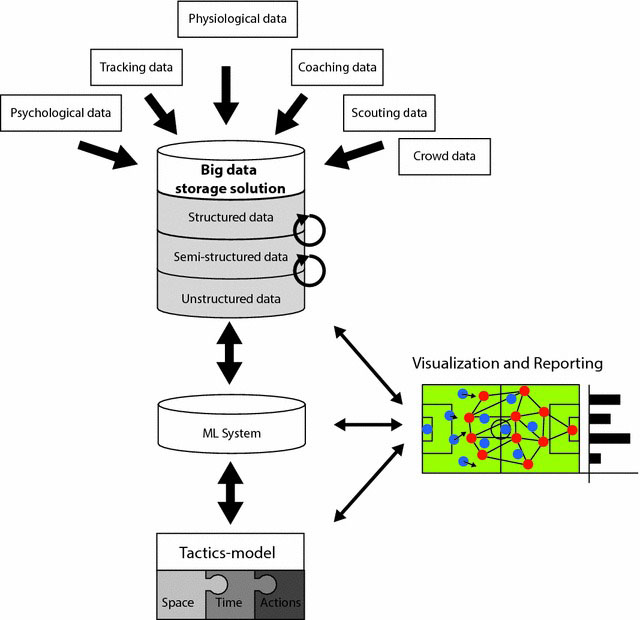
\includegraphics[width=8cm, height=8cm]{stack.jpg}
\cite{Rein2016}
\newline
First, the necessary infrastructure to collect the data is required. Second, a storage system is required allowing efficient data storage and access. Finally, a processing pipeline has to be established to extract relevant information from the data and to subsequently merge the information to build an explanatory and/or predictive model\cite{Rein2016}.An in-depth discussion of specific technological solutions is beyond the scope of the present study. A few useful technologies are however discussed, note we will only be discussing the software aspect since the hardware aspects have been discussed in great detail in the previous sections.\newline
It has previously been stressed upon how difficult it is to obtain the details of technologies clubs use to run their daily operations. However, after dissecting it is not all that difficult to make an educated guess on which tools could possibly be used for the above purposes. Let's start with obtaining data in the previous sections we have already seen how opta obtains its data using live analysis\cite{Bialik2014}. Now we shall explore a new tool called Twitter Heron, which can be used to obtain information from tweets.\newline
One of the problems with opta is that it may not cover leagues/tiers which are not profitable for it. However, football clubs generally have very enthusiastic fan bases and with Twitter being a very convenient social media tool we can try to mine data from tweets to generate our data. Twitter heron is a real-time analytics platform developed by Twitter. It is the direct successor of Apache Storm, built to be backward compatible with Storm's topology API but with a wide array of architectural improvements. Heron supports Seamless support for different processing semantics, is efficient and scales extremely well. A good blog on why Twitter heron is ideal can be found here.\cite{Ramasamy2000}\newline
Previously we touched on the subject of how scouts could use data from opta for analysis, from the internet the best way to obtain such data is to extract from XML. For this many different ways can be used. Some of the most popular manners are using Map Reduce, LogParser and even PIG.\newline
MapReduce is a processing technique and a program model for distributed computing based on java. The MapReduce algorithm contains two important tasks, namely Map and Reduce. The map takes a set of data and converts it into another set of data, where individual elements are broken down into tuples (key/value pairs). Secondly, reduce task, which takes the output from a map as an input and combines those data tuples into a smaller set of tuples. As the sequence of the name MapReduce implies, the reduce task is always performed after the map job.

The major advantage of MapReduce is that it is easy to scale data processing over multiple computing nodes. Under the MapReduce model, the data processing primitives are called mappers and reducers. Decomposing a data processing application into mappers and reducers is sometimes nontrivial. But, once we write an application in the MapReduce form, scaling the application to run over hundreds, thousands, or even tens of thousands of machines in a cluster is merely a configuration change. This simple scalability is what has attracted many programmers to use the MapReduce model.\cite{Tutorialspoint2000}\newline
Log Parser is a free command line utility for Windows that allows you to perform queries against a variety of file types including things like log files, CSV files, and XML files. This utility can even parse data sources such as the Active Directory or the Windows Event Logs.
Log Parser is extremely flexible, but it is not a utility for novices. Using Log Parser requires experience with custom queries as well as with working from the command line.
An example of PIG XML parsing can be found in this blog \cite{learnbigdataanalytics2000}.We can Use Spark SQL for querying data from DBs so that it can be used to extract features and clean up data. 

\section{Conclusions}

It can be seen the huge impact Big Data has in soccer. It has become a multi-million business. The acquisition of StatDNA by Arsenal for 2 million is proof of that. Also nowadays more and more clubs are being run entirely on big data proof of this is FC Midtjylland (Denmark) and also Brentford FC (England). Matthew Benham and Rasmus Ankersen are the pioneers in data analysis and have completely revolutionized their scouting departments. OPTA is the global leader in stats generation and is rated above 60 Million plus. Aside from just scouting potentials, it is used to shape tactics and also understand the strengths and weakness of players. While it may appear that the industry seems to have less scope of development this is only true for the top-ranked clubs. Most of the mid-table and lower league clubs still make use of traditional methods. The scope for open source software which provides a detailed scouting analysis has a huge market potential.

\bibliographystyle{ACM-Reference-Format}
\bibliography{report} 

\section{Bibtex Issues}
\todo[inline]{Warning--no number and no volume in Bialik2014}
\todo[inline]{Warning--page numbers missing in both pages and numpages fields in Bialik2014}
\todo[inline]{Warning--no number and no volume in cooling}
\todo[inline]{Warning--page numbers missing in both pages and numpages fields in cooling}
\todo[inline]{Warning--no number and no volume in learnbigdataanalytics2000}
\todo[inline]{Warning--page numbers missing in both pages and numpages fields in learnbigdataanalytics2000}
\todo[inline]{Warning--no number and no volume in 2012}
\todo[inline]{Warning--page numbers missing in both pages and numpages fields in 2012}
\todo[inline]{Warning--no number and no volume in Luca20000}
\todo[inline]{Warning--page numbers missing in both pages and numpages fields in Luca20000}
\todo[inline]{Warning--no number and no volume in 2000}
\todo[inline]{Warning--page numbers missing in both pages and numpages fields in 2000}
\todo[inline]{Warning--no number and no volume in Optasports2000}
\todo[inline]{Warning--page numbers missing in both pages and numpages fields in Optasports2000}
\todo[inline]{Warning--no number and no volume in Outsideoftheboot2000}
\todo[inline]{Warning--page numbers missing in both pages and numpages fields in Outsideoftheboot2000}
\todo[inline]{Warning--no number and no volume in Ramasamy2000}
\todo[inline]{Warning--page numbers missing in both pages and numpages fields in Ramasamy2000}
\todo[inline]{Warning--no number and no volume in Rein2016}
\todo[inline]{Warning--page numbers missing in both pages and numpages fields in Rein2016}
\todo[inline]{Warning--no number and no volume in Rejec2000s}
\todo[inline]{Warning--page numbers missing in both pages and numpages fields in Rejec2000s}
\todo[inline]{Warning--no number and no volume in Tutorialspoint2000}
\todo[inline]{Warning--page numbers missing in both pages and numpages fields in Tutorialspoint2000}
\todo[inline]{Warning--no number and no volume in wikipedia}
\todo[inline]{Warning--page numbers missing in both pages and numpages fields in wikipedia}
\todo[inline]{(There were 26 warnings)}
\section{Issues}

\subsection{Formatting}

    \done{Incorrect number of keywords or HID and i523 not included in the keywords}
    \done{Other formatting issues: No introduction?}



\subsection{Details about the Figures and Tables}

    \done{Capitalization errors in referring to captions, e.g. Figure 1, Table 2}

\section{Bibtex Issues}
\done[inline]{Warning--no number and no volume in Bialik2014}
\done[inline]{Warning--page numbers missing in both pages and numpages fields in Bialik2014}
\done[inline]{Warning--no number and no volume in cooling}
\done[inline]{Warning--page numbers missing in both pages and numpages fields in cooling}
\done[inline]{Warning--no number and no volume in learnbigdataanalytics2000}
\done[inline]{Warning--page numbers missing in both pages and numpages fields in learnbigdataanalytics2000}
\done[inline]{Warning--no number and no volume in 2012}
\done[inline]{Warning--page numbers missing in both pages and numpages fields in 2012}
\done[inline]{Warning--no number and no volume in Luca20000}
\done[inline]{Warning--page numbers missing in both pages and numpages fields in Luca20000}
\done[inline]{Warning--no number and no volume in 2000}
\done[inline]{Warning--page numbers missing in both pages and numpages fields in 2000}
\done[inline]{Warning--no number and no volume in Optasports2000}
\done[inline]{Warning--page numbers missing in both pages and numpages fields in Optasports2000}
\done[inline]{Warning--no number and no volume in Outsideoftheboot2000}
\done[inline]{Warning--page numbers missing in both pages and numpages fields in Outsideoftheboot2000}
\done[inline]{Warning--no number and no volume in Ramasamy2000}
\done[inline]{Warning--page numbers missing in both pages and numpages fields in Ramasamy2000}
\done[inline]{Warning--no number and no volume in Rein2016}
\done[inline]{Warning--page numbers missing in both pages and numpages fields in Rein2016}
\done[inline]{Warning--no number and no volume in Rejec2000s}
\done[inline]{Warning--page numbers missing in both pages and numpages fields in Rejec2000s}
\done[inline]{Warning--no number and no volume in Tutorialspoint2000}
\done[inline]{Warning--page numbers missing in both pages and numpages fields in Tutorialspoint2000}
\done[inline]{Warning--no number and no volume in wikipedia}
\done[inline]{Warning--page numbers missing in both pages and numpages fields in wikipedia}
\done[inline]{(There were 26 warnings)}
\end{document}
